\documentclass[]{article}
\usepackage[spanish.mexico]{babel}
\usepackage[T1]{fontenc}
\usepackage[utf8]{inputenc}
\usepackage{lmodern}
\usepackage[a4paper]{geometry}

%Multimagen
\usepackage{subcaption}

%texto Imagen
\usepackage{sidecap}

\usepackage{hyperref}
%Enclaces
\hypersetup{
	colorlinks=true,
	linkcolor=blue,
	filecolor=magenta,      
	urlcolor=cyan,
}

\urlstyle{same}

\usepackage{graphicx}
\usepackage{cite}

%DIAGRAMA DE GANT 
\usepackage{pgfgantt}
%\usepackage{graphicx}
\usepackage{xcolor}
%\usepackage[spanish.mexico]{babel}
%\usepackage[utf8]{inputenc}
%\usetikzlibrary{positioning}

\ganttset{group/.append style={orange},
	milestone/.append style={red},
	progress label node anchor/.append style={text=red}}

%%MULTICOL


\usepackage{etoolbox,refcount}
\usepackage{multicol}

\newcounter{countitems}
\newcounter{nextitemizecount}
\newcommand{\setupcountitems}{%
	\stepcounter{nextitemizecount}%
	\setcounter{countitems}{0}%
	\preto\item{\stepcounter{countitems}}%
}
\makeatletter
\newcommand{\computecountitems}{%
	\edef\@currentlabel{\number\c@countitems}%
	\label{countitems@\number\numexpr\value{nextitemizecount}-1\relax}%
}
\newcommand{\nextitemizecount}{%
	\getrefnumber{countitems@\number\c@nextitemizecount}%
}
\newcommand{\previtemizecount}{%
	\getrefnumber{countitems@\number\numexpr\value{nextitemizecount}-1\relax}%
}
\makeatother    
\newenvironment{AutoMultiColItemize}{%
	\ifnumcomp{\nextitemizecount}{>}{3}{\begin{multicols}{2}}{}%
		\setupcountitems\begin{itemize}}%
		{\end{itemize}%
		\unskip\computecountitems\ifnumcomp{\previtemizecount}{>}{3}{\end{multicols}}{}}


\title{Presentación de productos IDEA 1.61}
\author{Pablo Vivar Colina}
%\date{October 2015}




\begin{document}

%%\usepackage[top=2cm,bottom=2cm,left=1cm,right=1cm]{geometry}
\begin{titlepage}
     \begin{center}
	
\includegraphics[width=0.1\textwidth]{UNAM}
        \Large Universidad Nacional Autónoma de México
        	
\includegraphics[width=0.1\textwidth]{FI}\\[1cm]
        \Large Facultad de Ingeniería\\[1cm]
        \Large Arduino UNO\\[1cm]
        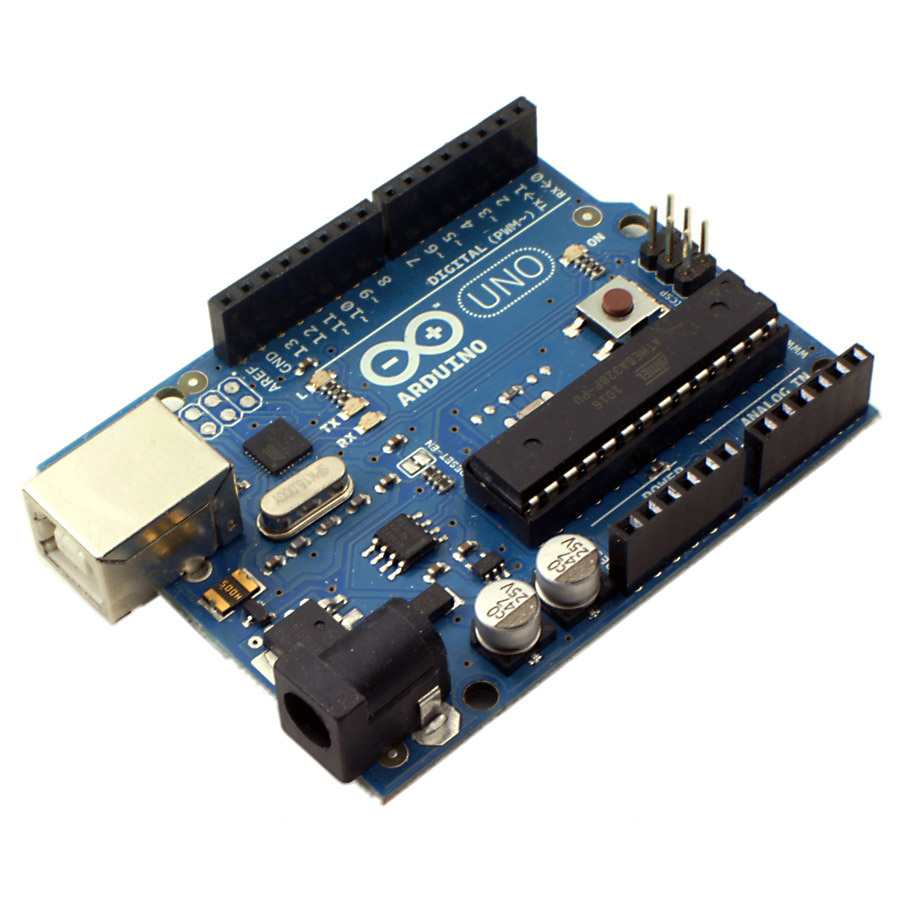
\includegraphics[width=0.6\textwidth]{Arduino_Uno_Angle}\\[1cm]
         %\Large Laboratorio de Acústica y Óptica (4314)\\[1cm]
         %\footnotesize Profesor: Bañuelos Saucedo Miguel Ángel M.I.\\[1cm]
        \footnotesize Semestre 2016-2\\[1cm]
        \Large Elaboración de sistema electromecánico\\[1cm]
        %\Large Reflexión y Refracción\\[1cm]
        \end{center}
         %Texto a la derecha
          \begin{flushright}
%\footnotesize  Grupo 05\\[0.5cm]
%\footnotesize Brigada: 4\\[0.5cm]
%\footnotesize Integrantes:\\[0.5cm]
%\footnotesize Brihuega Razo Ximena Biviana\\[0.5cm]
%\footnotesize Martínez Carsolio Rodolfo\\[0.5cm]
\footnotesize Vivar Colina Pablo\\[0.5cm]
 \end{flushright}
    %Texto a la izquierda
          \begin{flushleft}
        \footnotesize Ciudad Universitaria a Febrero 2016.\\
          \end{flushleft}
         
          
        %\vfill
        %\today
    \end{center}
\end{titlepage} 

\maketitle

\begin{center}
	
\includegraphics[width=0.2\textwidth]{idea.png}
\end{center}


\section{Impresión 3D}

Ve tu diseño convertirse en realidad al imprimirlo en 3D. Nuestras máquinas ocupan tecnología de Fused Deposition Modeling (FDM) para obtener la mejor calidad al mejor precio. Todas las impresiones son totalmente personalizadas.\\

\section{Ditac}

Ditac es un sistema de construcción hecho con piezas de acrílico cortadas mediante tecnología láser de gran precisión, éstas puedan ser utilizadas para entretenimiento o para la elaboración de prototipos de mecatrónica.\\


\begin{figure}[h!]
	\centering
	\begin{subfigure}[b]{0.3\textwidth}
		\includegraphics[width=1\textwidth]{piezasRTM}
		%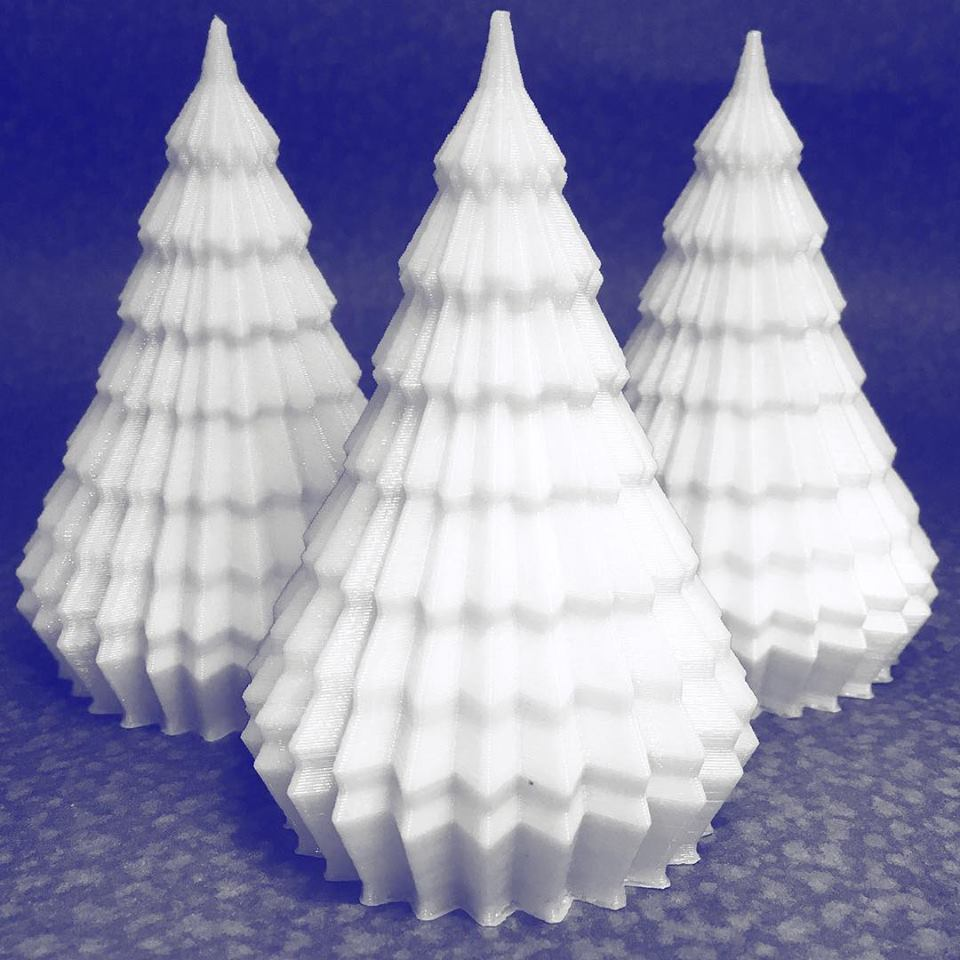
\includegraphics[]{arboles1}		
		\caption{Piezas}
		%\label{fig:VoltCorr}
	\end{subfigure}
	~ %add desired spacing between images, e. g. ~, \quad, \qquad, \hfill etc. 
	%(or a blank line to force the subfigure onto a new line)
	\begin{subfigure}[b]{0.3\textwidth}	
		
\includegraphics[width=1\textwidth]{LogoDitacReg}
		%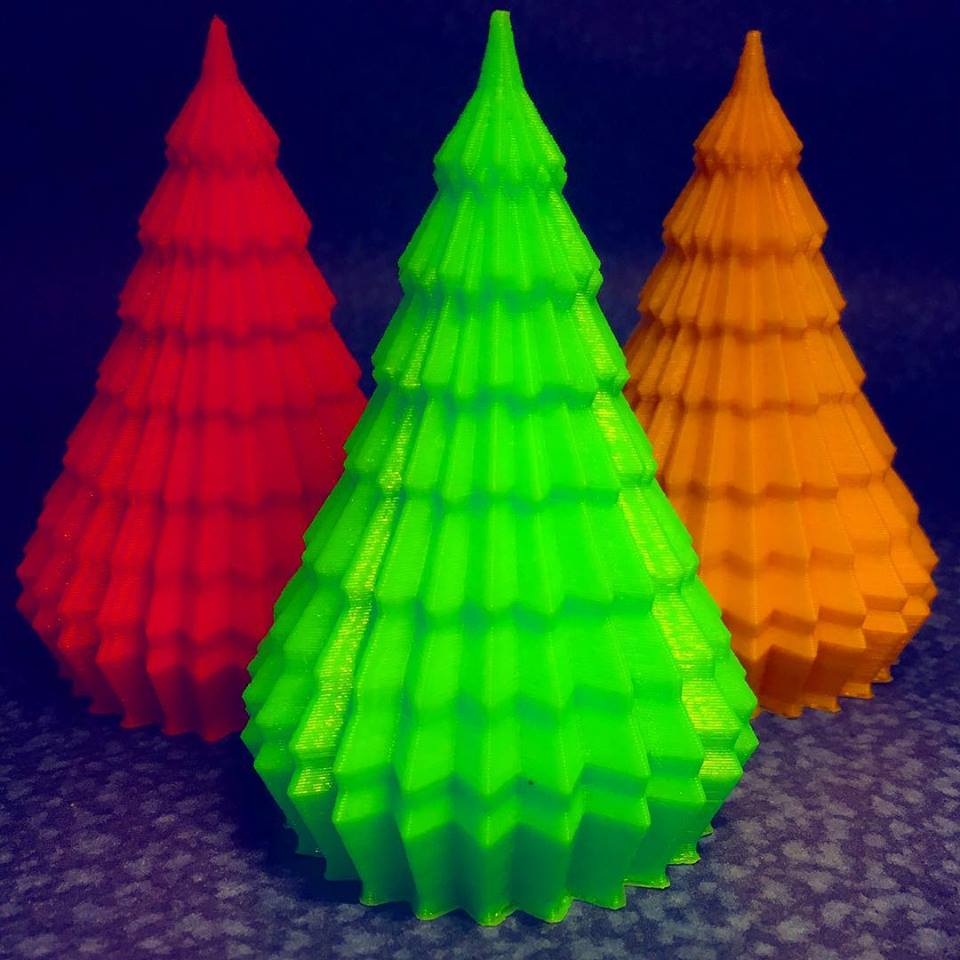
\includegraphics[]{arboles2}
		\caption{Logo Ditac (MR)}
		%\label{fig:ResComp}
	\end{subfigure}
	~ %add desired spacing between images, e. g. ~, \quad, \qquad, \hfill etc. 
%(or a blank line to force the subfigure onto a new line)
	\begin{subfigure}[b]{0.3\textwidth}
		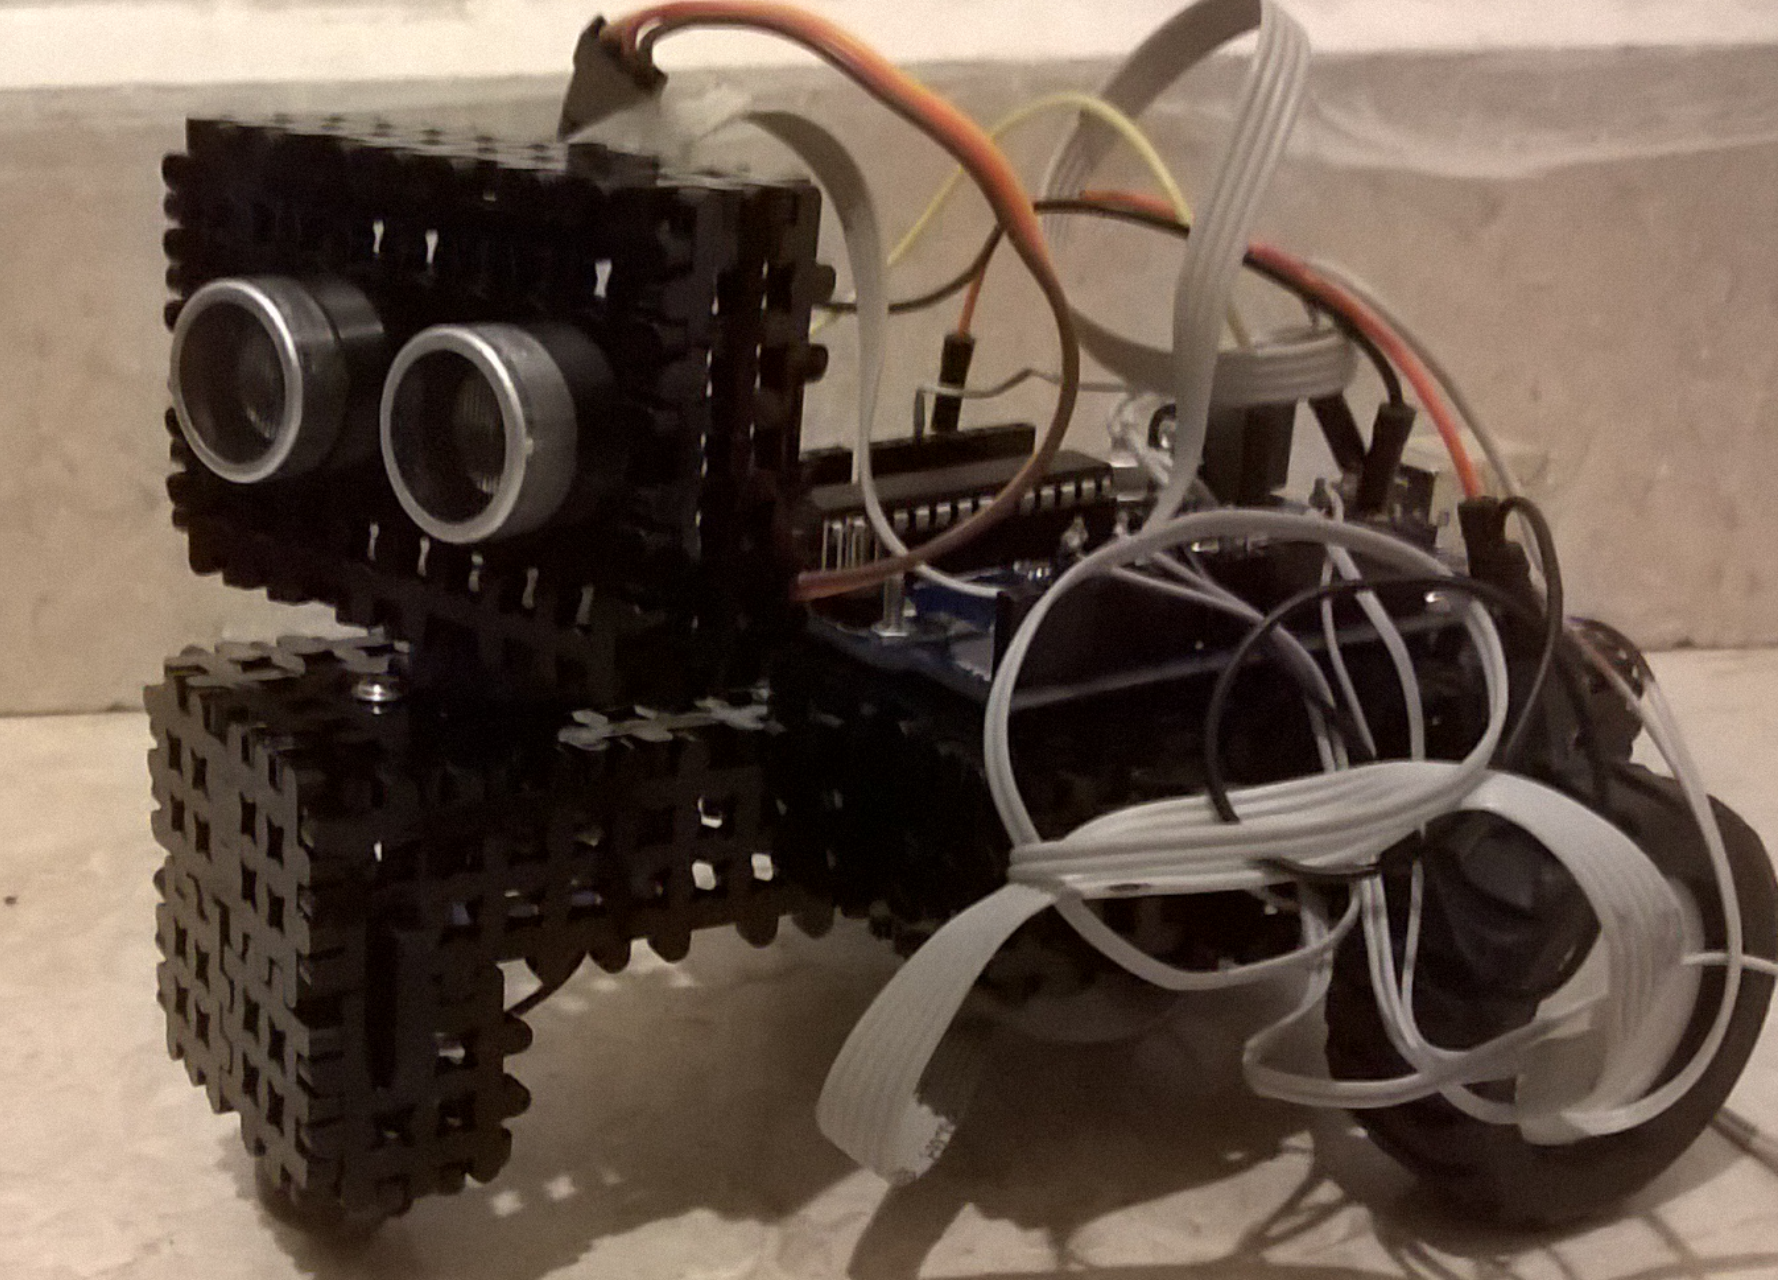
\includegraphics[width=1\textwidth]{mecaRTM}	
		\caption{Robot}
		%\label{fig:PortaLlaves}
	\end{subfigure}

	\caption{Fotos Ditac}
	\label{fig:Ditac}
\end{figure}



\section{Diseño}

Ya hiciste lo más difícil…. tener una IDEA. Déjanos ayudarte a plasmarla en la computadora, para que se pueda imprimir correctamente. Creamos diseños innovadores por medio de software Diseño Asistido por Computador (CAD) como por ejemplo: Parametric Creo, OpenSCAD, SolidWorks, Blender.\\

\section{Desarrollo de Proyectos}

Tu que quieres quieres crear algo, no te preocupes por los detalles. Nosotros podemos asistirte con tus proyectos escolares al igual que profesionales. Contamos con un equipo de ingenieros especializados en diferentes ramas para asegurar la más alta calidad en tu proyecto.\\

\section{Comunidad}

“Si quieres llegar rápido, ve solo. Pero si quieres llegar lejos, ve acompañado.” En IDEA 1.61, promovemos la colaboración por lo cual desarrollamos contenido libre.\\

\section{Mecánica y Electrónica}

Contamos con componentes mecanicos y electricos para tu proyecto a bajo costo. Al comprar con nosotros, damos apoyo y guía para usar los componentes.\\

\section{Concepto de empresa}
 
Empresa dedicada a la innovación y tecnología, especializada en ofrecer un espacio para desarrollar ideas y proyectos mediante el uso de máquinas de diseño (Impresoras 3D, CNC, cortadora laser) y herramientas de mecánica y electrónica.\\

\subsection{Misión}
 
Ofrecer un espacio de aprendizaje y difusión de innovación, al proveer acceso a máquinas de diseño, contribuyendo al desarrollo de nuevas tecnologías para el beneficio de futuras generaciones.\\


\subsection{Visión}
 
Ser líderes promotores del desarrollo de tecnología de vanguardia, creando una comunidad global de innovadores.\\

\subsection{Valores}

\begin{enumerate}
	\item Mejora continua todos los días, en todas las actividades y proyectos que se realicen.
	\item Honestidad  con todos, empezando por nosotros mismos.
	\item Servicio al cliente de calidad y en excelencia.
	\item Compromiso para hacer posibles las nuevas ideas.
	\item Trabajo en equipo para alcanzar los objetivos planteados.
	\item Liderazgo para ofrecer siempre el mejor servicio, con las mejores herramientas.
	\item Responsabilidad con la empresa, con la sociedad y en nuestra vida personal.
	\item Pasión hacia nuestra misión y visión, para el desarrollo de nuevas tecnologías.
	\item Unidad entre nuestra comunidad, para crear una familia de innovadores que transformen al mundo. 	 
\end{enumerate} 



\section{Biomateriales (PLA)}

Es el material recomendado por muchas compañías fabricantes de impresoras 3D de escritorio, el PLA cumple con una amplia gama de aplicaciones para impresión, además de ser un material ecológico formado con recursos renovables como el almidón de maíz y requiere menos energía para procesar plásticos.\\

\section{Productos}

A través de las nuevas tecnologías como las impresoras 3D y las máquinas de corte láser hacemos distribución de productos como cajas para eventos especializadas y objetos ornamentales.\\

Éste tipo de tecnologías resulta muy versátil en la elaboración de nuevos productos, por lo que ponemos a su disposición la elaboración de cajas MDF por pedido, y tambien de zouvenirs con el sistema de construcción DITAC.\\ 

\begin{figure}[h!]
	\centering
	\begin{subfigure}[b]{0.4\textwidth}
			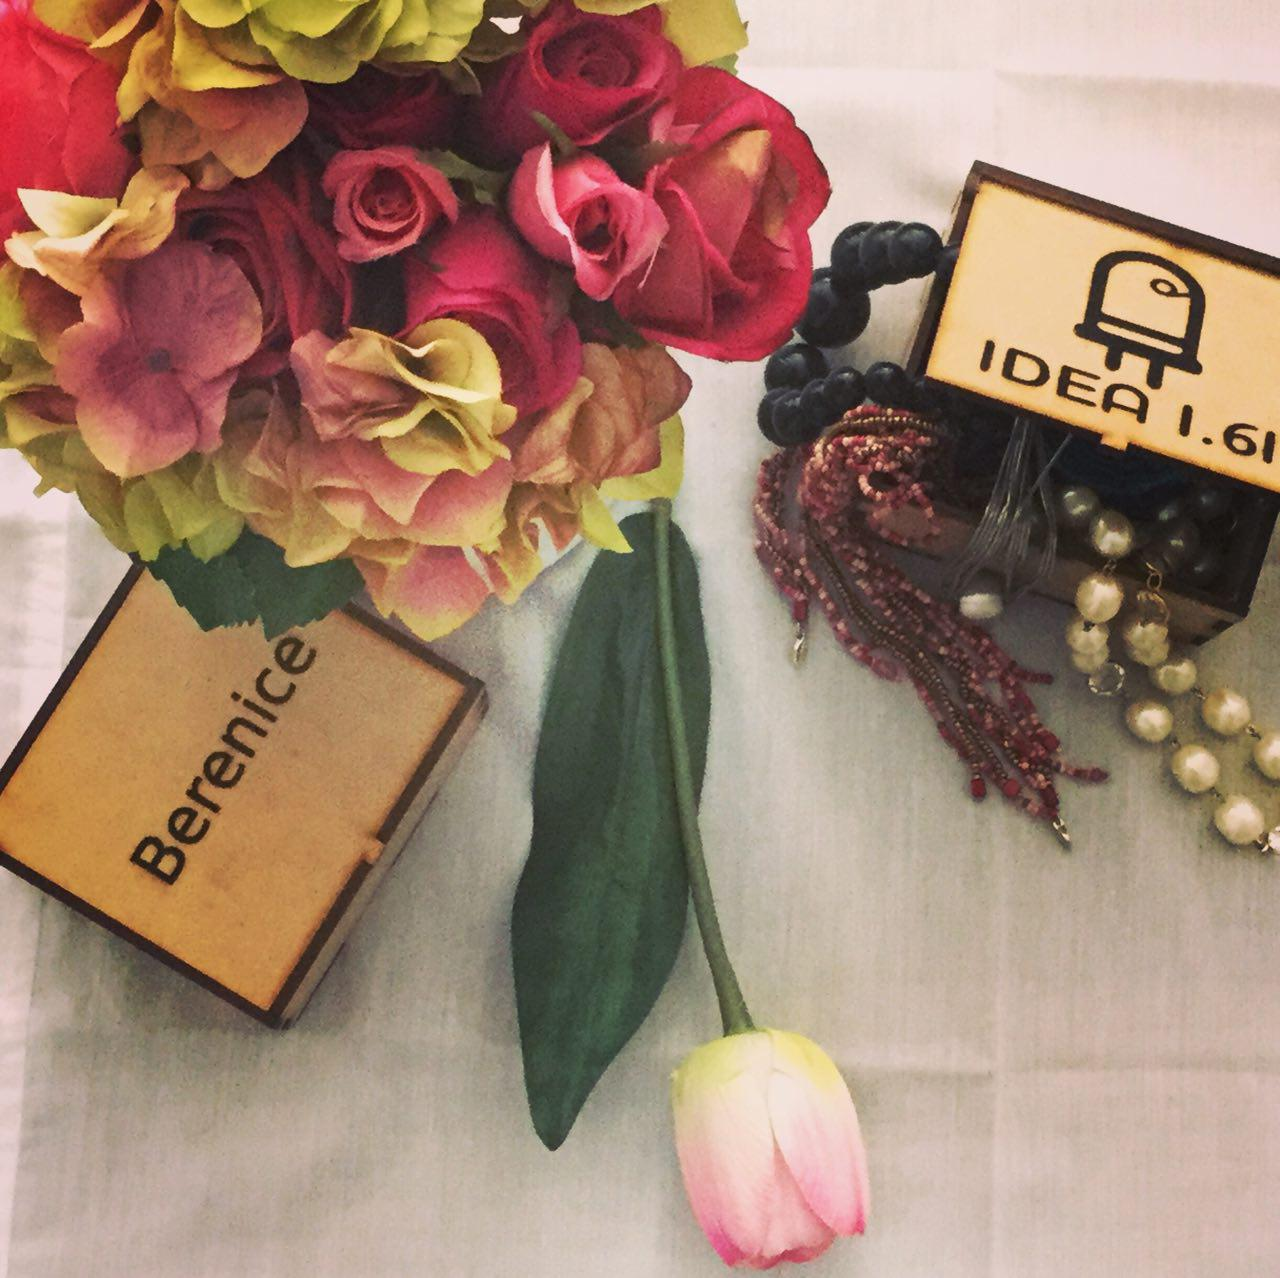
\includegraphics[width=1\textwidth]{CajasPersonalizadas}
		%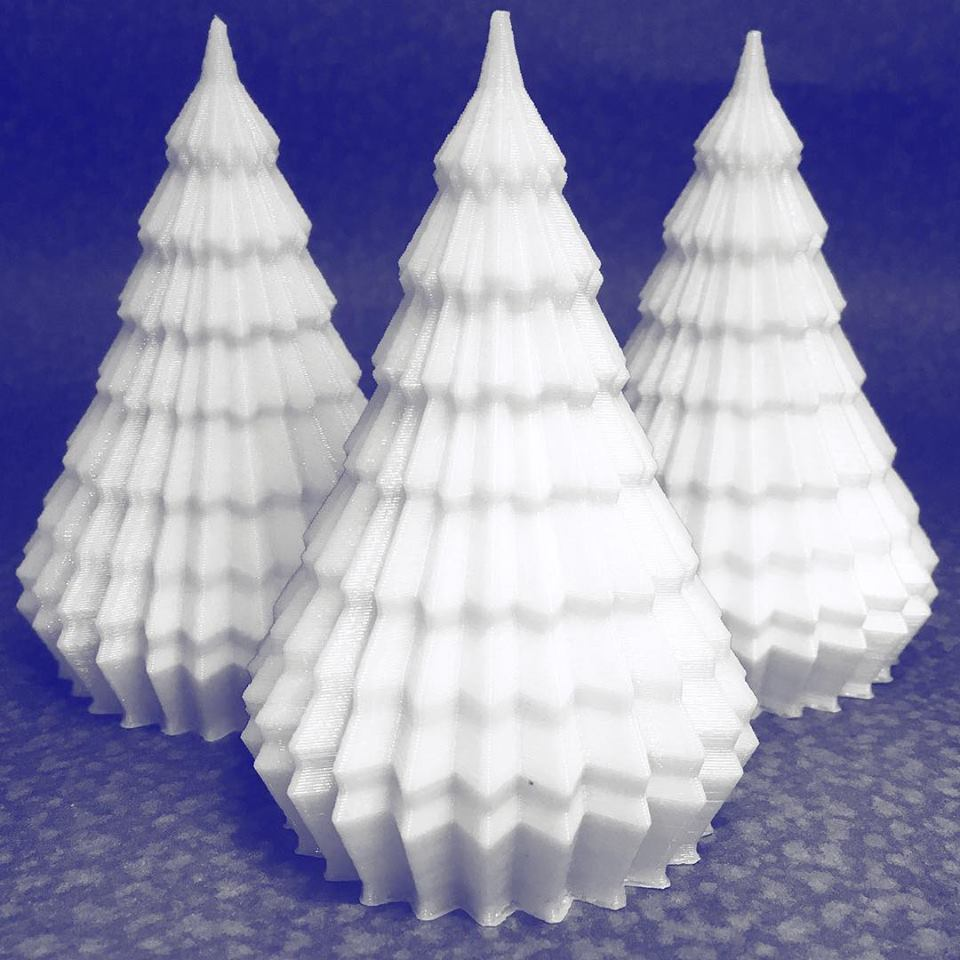
\includegraphics[]{arboles1}		
		%\caption{}
		%\label{fig:VoltCorr}
	\end{subfigure}
	~ %add desired spacing between images, e. g. ~, \quad, \qquad, \hfill etc. 
	%(or a blank line to force the subfigure onto a new line)
	\begin{subfigure}[b]{0.4\textwidth}	
		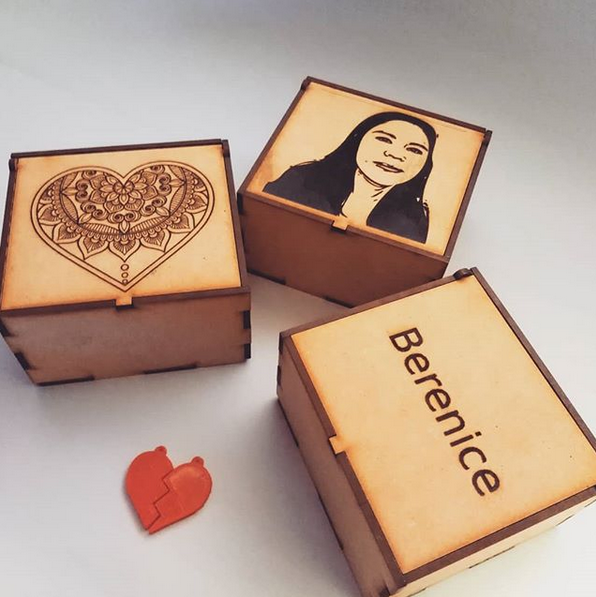
\includegraphics[width=0.75\textwidth]{AmorAmistad}
		%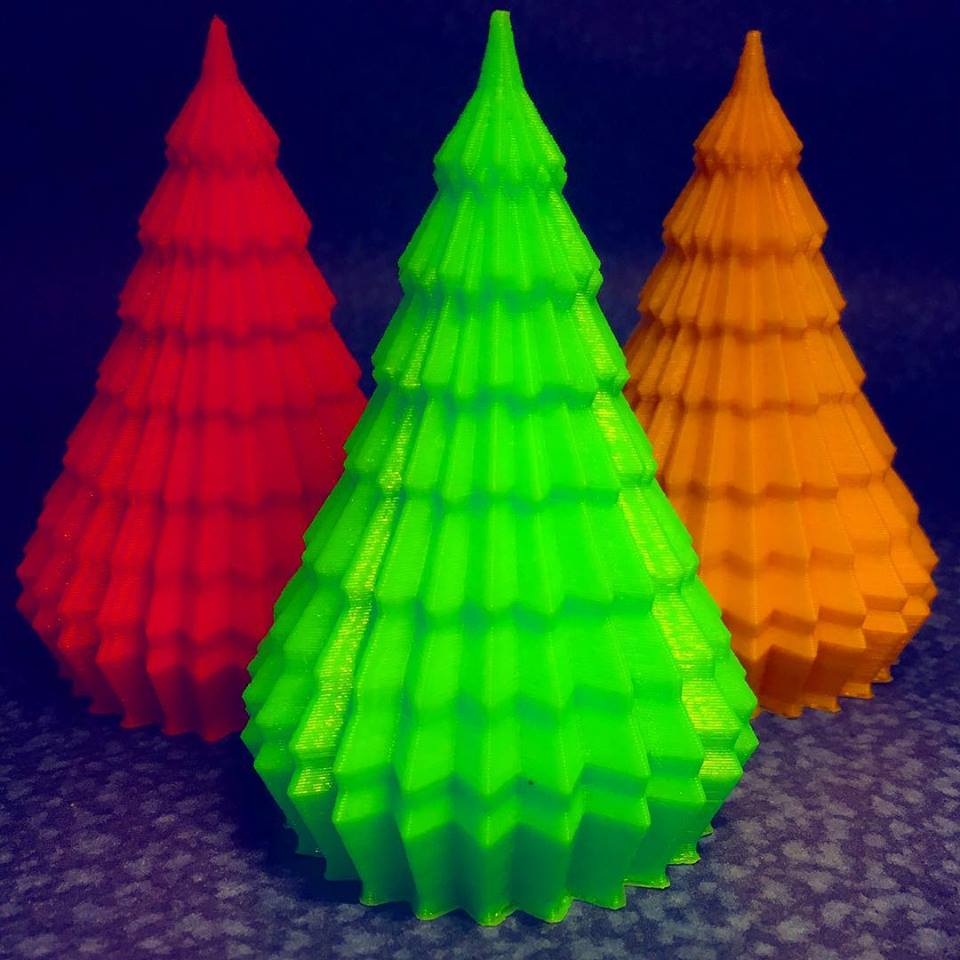
\includegraphics[]{arboles2}
		%\caption{Decoración PLA}
		%\label{fig:ResComp}
	\end{subfigure}
	\caption{Caja standard MDF}
    \label{fig:cajaStdMDF}
\end{figure}

\begin{figure}[h!]
	\centering
	\begin{subfigure}[b]{0.4\textwidth}
		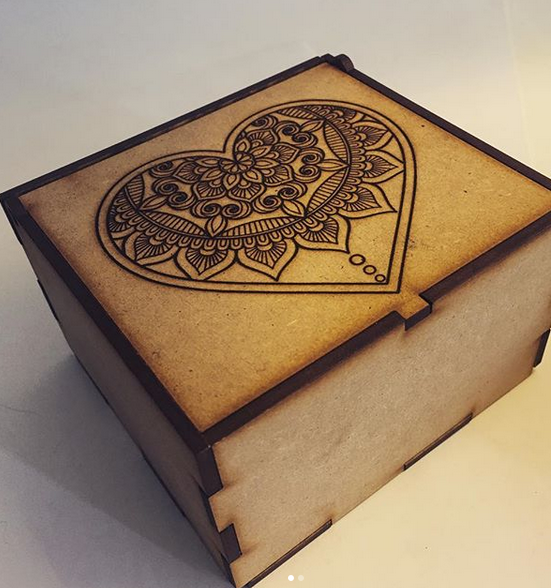
\includegraphics[width=0.85\textwidth]{AmorAmistad2}
		%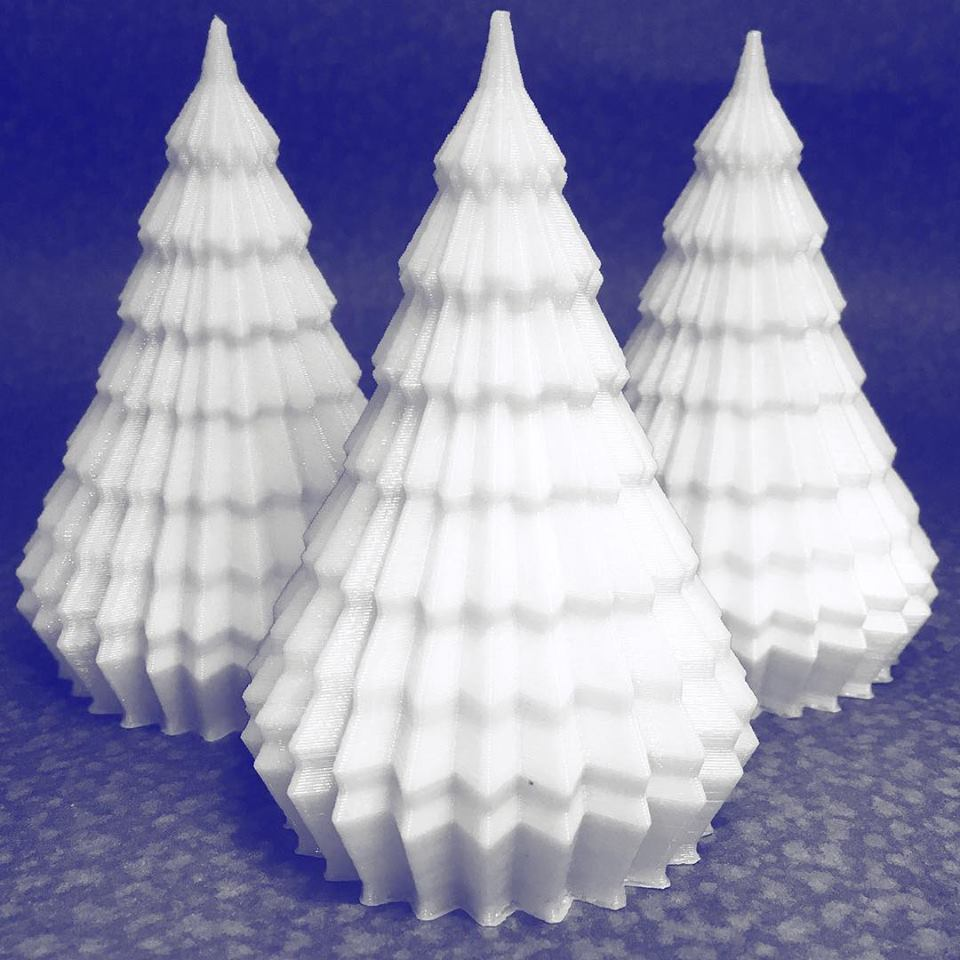
\includegraphics[]{arboles1}		
		%\caption{}
		%\label{fig:VoltCorr}
	\end{subfigure}
	~ %add desired spacing between images, e. g. ~, \quad, \qquad, \hfill etc. 
	%(or a blank line to force the subfigure onto a new line)
	\begin{subfigure}[b]{0.4\textwidth}	
			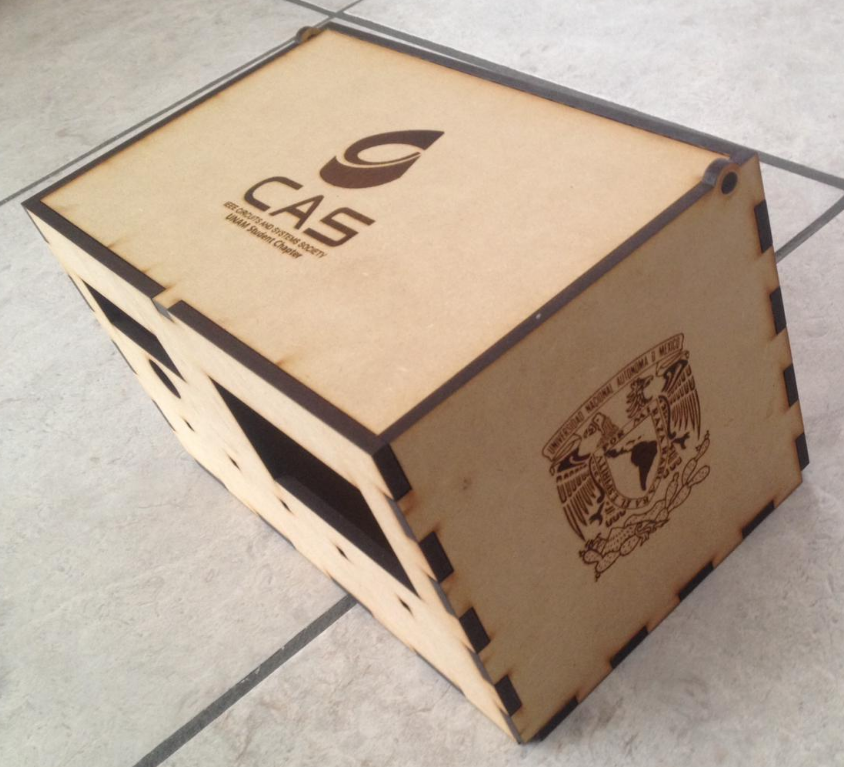
\includegraphics[width=1\textwidth]{caseCAS}
		%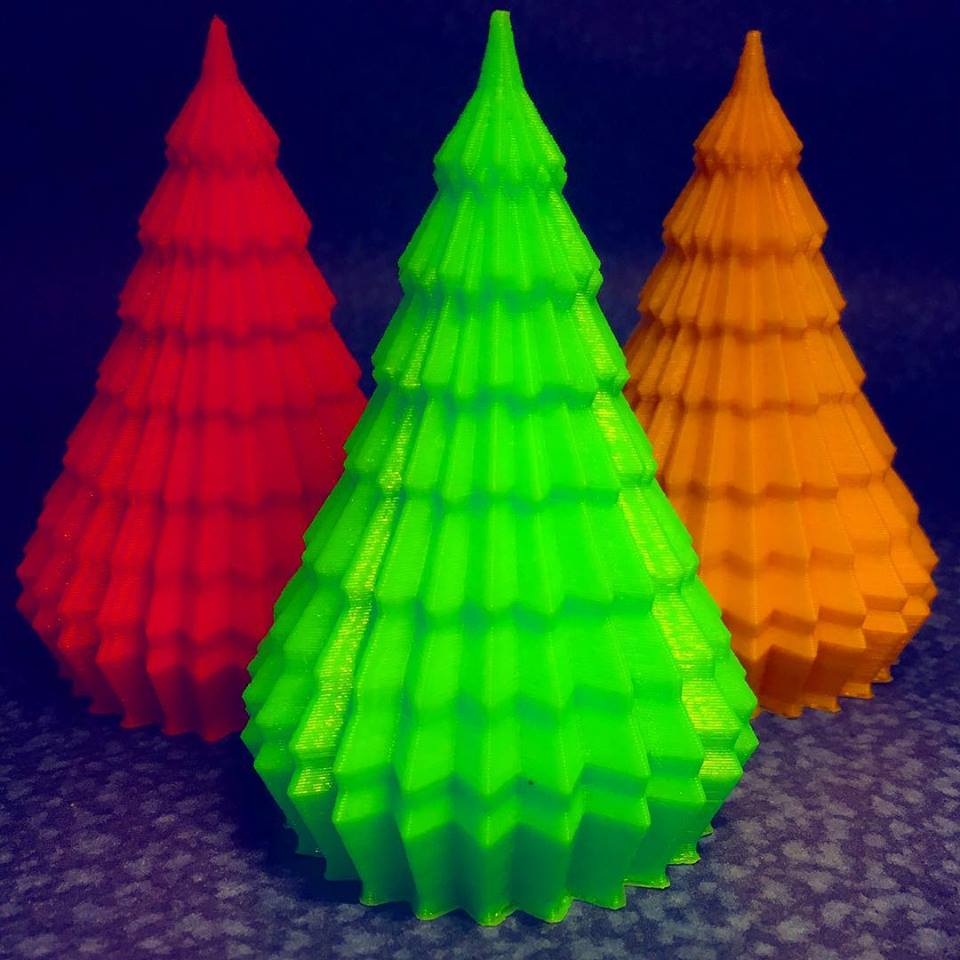
\includegraphics[]{arboles2}
		%\caption{Decoración PLA}
		%\label{fig:ResComp}
	\end{subfigure}
	\caption{Cajas MDF a la medida}
	\label{fig:cajaMDFV2}
\end{figure}

\begin{figure}[h!]
	\centering
	\begin{subfigure}[b]{0.4\textwidth}
			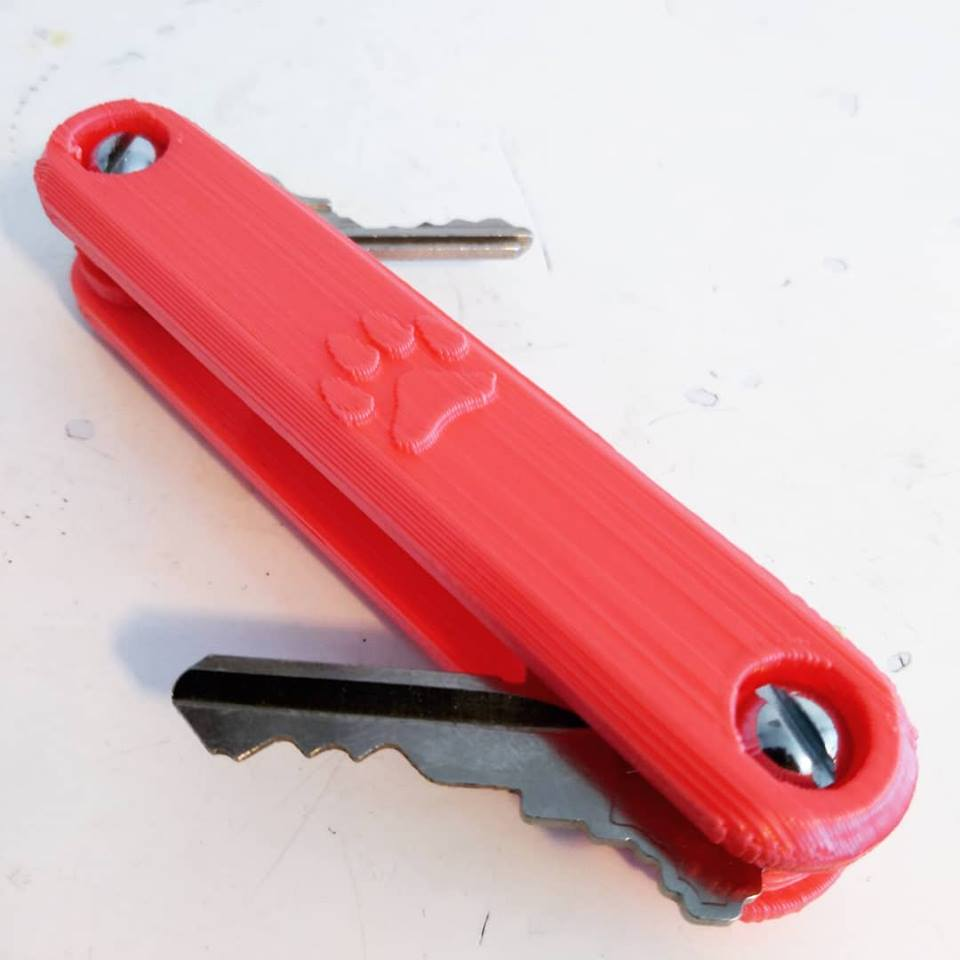
\includegraphics[width=1\textwidth]{portallaves}	
		\caption{Porta Llaves}
	\label{fig:PortaLlaves}
	\end{subfigure}
	~ %add desired spacing between images, e. g. ~, \quad, \qquad, \hfill etc. 
	%(or a blank line to force the subfigure onto a new line)
	\begin{subfigure}[b]{0.4\textwidth}	
		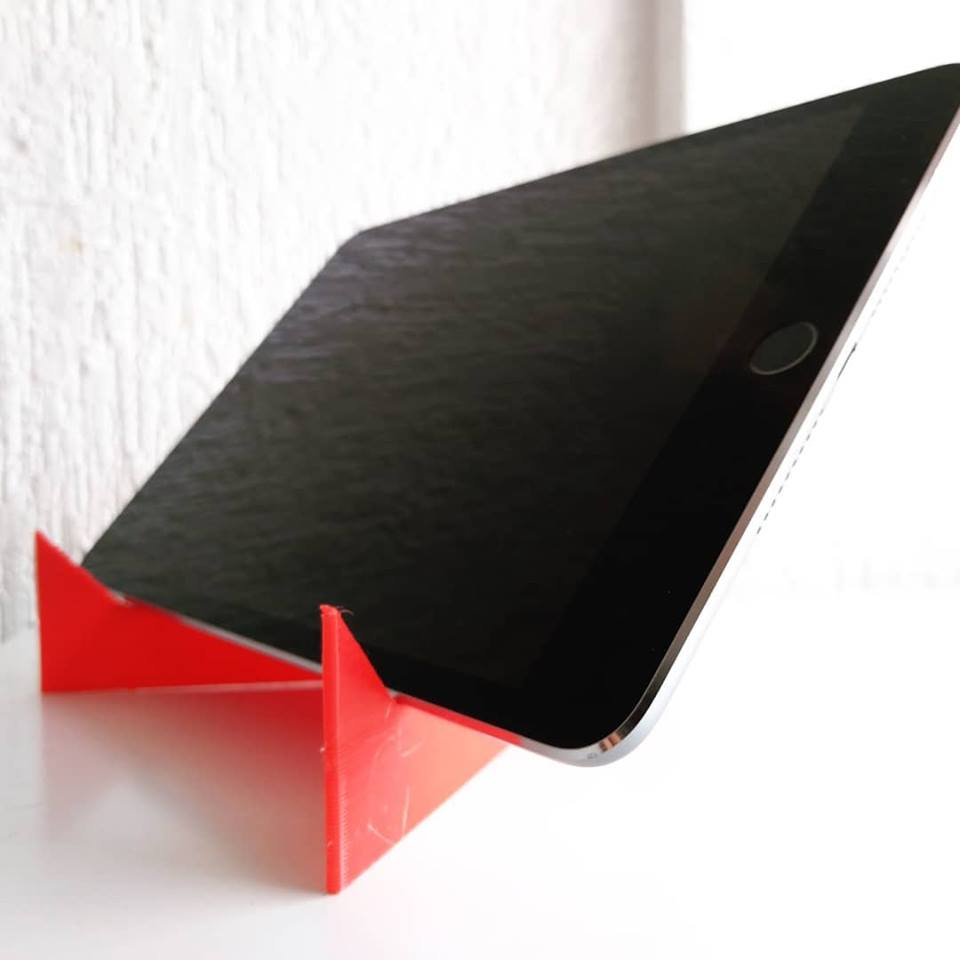
\includegraphics[width=1\textwidth]{stand1}
		\caption{Stand Tablet}
		\label{fig:StandTablet}
	\end{subfigure}
	\caption{Objetos Utilitarios}
	\label{fig:utilidad3D}
\end{figure}

\begin{figure}[h!]
	\centering
	\begin{subfigure}[b]{0.4\textwidth}
		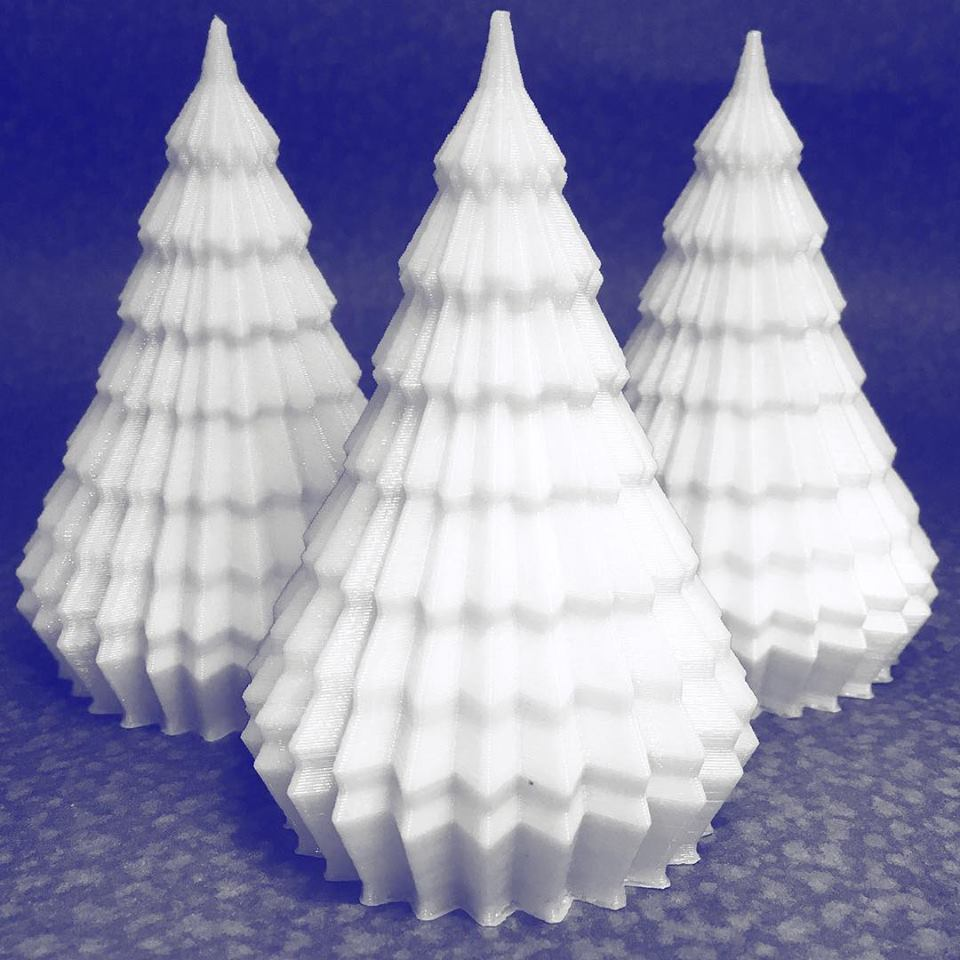
\includegraphics[width=1\textwidth]{arboles1}
		%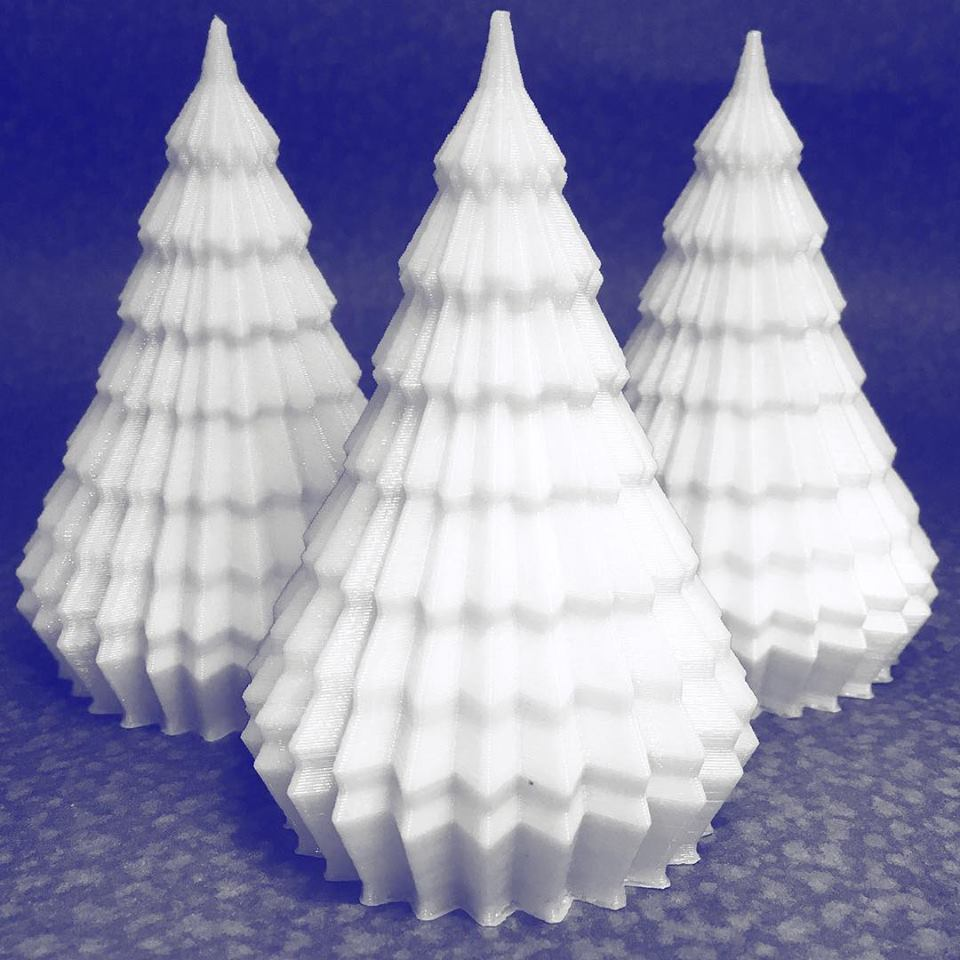
\includegraphics[]{arboles1}		
		%\caption{}
		%\label{fig:VoltCorr}
	\end{subfigure}
	~ %add desired spacing between images, e. g. ~, \quad, \qquad, \hfill etc. 
	%(or a blank line to force the subfigure onto a new line)
	\begin{subfigure}[b]{0.4\textwidth}	
		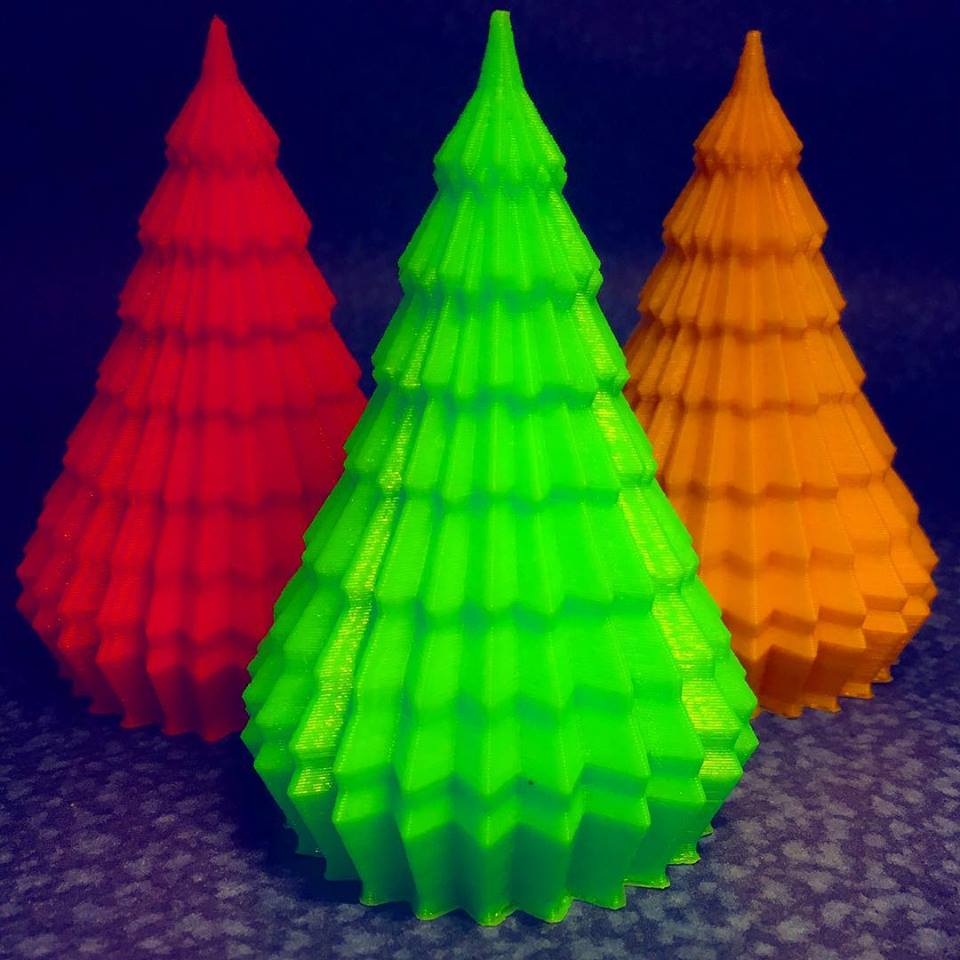
\includegraphics[width=1\textwidth]{arboles2}
		%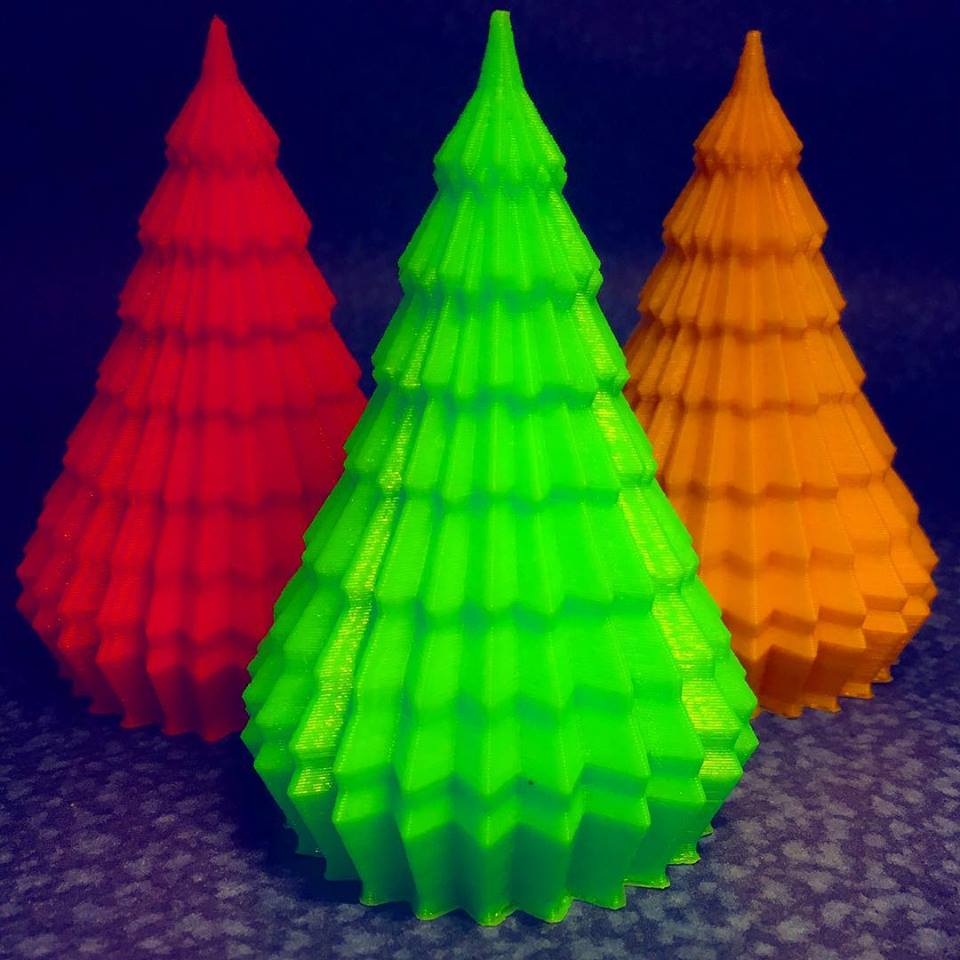
\includegraphics[]{arboles2}
		%\caption{Decoración PLA}
		%\label{fig:ResComp}
	\end{subfigure}
	\caption{Decoración Impresa en 3D}
	\label{Fig:decoracionPLA}
\end{figure}

%\begin{figure}[h!]
%	\centering
%	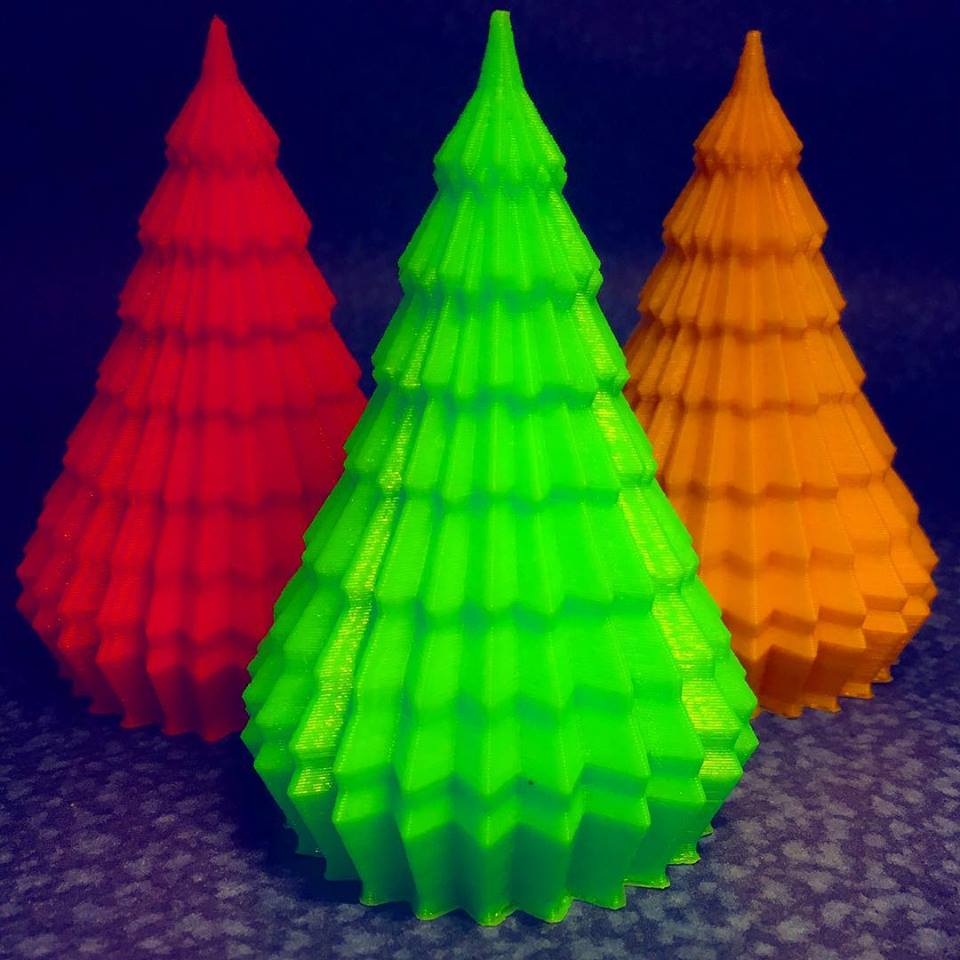
\includegraphics[width=0.5\textwidth]{arboles2}
%		\caption{Decoración PLA}
%	\label{}
%\end{figure}

\begin{table}[h!]
	\centering
	\begin{tabular}{|c|c|c|}
		\hline
		\textbf{Modelo}    & \textbf{Costo 1 Pieza} & \textbf{Costo 10 Piezas}      \\ \hline
		\href{https://idea161.org/producto/caja-mdf-personalizada/}{Caja Standard MDF (fig \ref{fig:cajaStdMDF})}  & 45.6 & 36.2 \\ \hline 
			\href{https://idea161.org/producto/porta-llaves-impreso-3d/}{Portallaves (fig \ref*{fig:PortaLlaves})}  & 64.2 & 23.38\\ \hline 
		%	\href{https://www.idea161.org/productos}{Soporte Tablet (fig \ref{fig:StandTablet})}  & 23.38  & 1 \\ \hline 
		%	\href{https://www.idea161.org/productos}{Caja a Medida MDF (fig \ref{fig:cajaMDFV2})}  & 35.67 & 23.38 \\ \hline 
			\href{https://idea161.org/servicios/}{Soporte Tablet}  & 65  & 45 \\ \hline 
		
		
	\end{tabular}
	\caption{Precios productos}
	\label{precios}
\end{table}

En el cuadro \ref{precios} se enlistan los precios de los productos que se tienen actualmente en la página de 	\href{https://www.idea161.org}{IDEA 1.61}.\\



%\bibliographystyle{plain}
%\bibliography{referencias.bib}


\end{document}
